% ****** Start of file aipsamp.tex ******
%
%   This file is part of the AIP files in the AIP distribution for REVTeX 4.
%   Version 4.1 of REVTeX, October 2009
%
%   Copyright (c) 2009 American Institute of Physics.
%
%   See the AIP README file for restrictions and more information.
%
% TeX'ing this file requires that you have AMS-LaTeX 2.0 installed
% as well as the rest of the prerequisites for REVTeX 4.1
%
% It also requires running BibTeX. The commands are as follows:
%
%  1)  latex  aipsamp
%  2)  bibtex aipsamp
%  3)  latex  aipsamp
%  4)  latex  aipsamp
%
% Use this file as a source of example code for your aip document.
% Use the file aiptemplate.tex as a template for your document.
\documentclass[%
 aip,
 jmp,%
 amsmath,amssymb,
%preprint,%
 reprint,%
%author-year,%
%author-numerical,%
]{revtex4-1}

\usepackage{graphicx}% Include figure files
\usepackage{dcolumn}% Align table columns on decimal point
\usepackage{bm}% bold math
%\usepackage[mathlines]{lineno}% Enable numbering of text and display math
%\linenumbers\relax % Commence numbering lines

\begin{document}

\preprint{AIP/123-QED}

\title[]{Confinement Induced Electron Capture}

\author{C. Martin}
 \altaffiliation[Also at ]{Physics Department, XYZ University.}%Lines break automatically or can be forced with \\
\author{R. Godes}%
 \email{Second.Author@institution.edu.}
\affiliation{ 
Authors' institution and/or address%\\This line break forced with \textbackslash\textbackslash
}%


\date{\today}% It is always \today, today,
             %  but any date may be explicitly specified

\begin{abstract}
We describe a Gedandkenexperiment in which a bare proton can capture an electron due solely to confinement. We first briefly review the aspects around bare electron proton capture.  We then provide a numerical solution of the Fermi VA-Theory for electron capture for an electron-proton pair confined in a classical box of size L. Interestingly, we find that the capture is most likely for L=0.004-0.009 Angstroms, well beyond the radius of the proton and the Compton wavelength of the electron.  We also examine the implications for theoretical minimal power output for such a process.
%
\end{abstract}

\pacs{Valid PACS appear here}% PACS, the Physics and Astronomy
                             % Classification Scheme.
\keywords{Suggested keywords}%Use showkeys class option if keyword
                              %display desired
\maketitle

\section{\label{sec:level1}Background}

We briefly review orbital electron capture and some considerations, like environmental effects on the rate, that motivate this study.

\subsection{\label{sec:level2}Orbital Electron Capture}
In 1935, Yukawa proposed that a proton, bound in an atomic nucleus,  could capture a low lying, bound atomic electron, transforming into a neutron, and releasing an electron neutrino.


$$p^{+}+\;e^{-}\rightarrow\;n^{0}\;+\;\nu^{e}$$

This may be called orbital electron capture, K-electron capture, or just electron capture (E.C.) 

Electron capture usually occurs in unstable radioisotopes which lack the nuclear binding energy $Q$ to decay by the more familiar Beta decay processes ($\beta^{-}, \beta^{+}$). The typical $Q$ energies necessary are 

$$Q_{\beta^{+}}\sim2-4{MeV},\;\\;Q_{\beta^{-}}\sim0.5-2(MeV),\;\;{and}\;\;Q_{E.C.}\sim0.2-2.0{MeV}$$

When $Q<1.02{MeV}$, which is $2m_{e}c^{2}$, a proton rich nucleus must decay by electron capture.  Otherwise, all 3 processes compete.

In particular, heavy elements may decay by E.C. and/or $\beta^{+}$ (positron emission) to a lower 'magic number' of stable nuclei, and by $\beta^{-}$ decay to achieve a higher magic number.    E.C. is favored for high Z nuclei, but because of the energetic constraint, very light elements, such as $^{7}Be$ decay by primarily by E.C.    Lacking any binding energy, bare proton electron capture is not observed, and requires extreme, exotic conditions.
 
We observe electron capture by observing the resulting transmuted nuclei and/or the radiative relaxation processes.  The captured electron is bound to the atom, and it is usually a K-shell electron, but may be L or higher.  The nucleus may then absorb some energy, becoming excited, and then undergo internal conversion.  During this, another higher lying, bound atomic electron is absorbed, and either an X-ray or Auger electron released [see Figure \ref{fig:ec1}].

\begin{figure}
   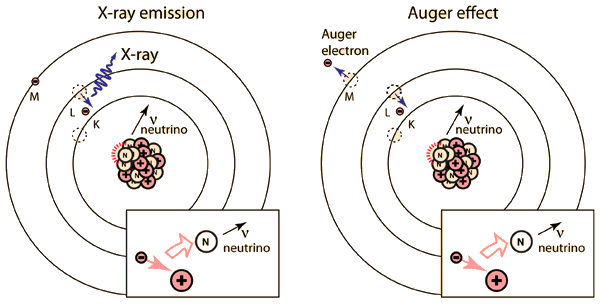
\includegraphics[scale=0.25]{img/ecrelax.png}
   \caption{orbital electron capture relaxation processes}
  \label{fig:ec1}
\end{figure}

Because electron capture occurs in proton-rich nuclei, and, subsequently, releases a X-Ray photon, the reaction is also sometimes written as

$$^{Z}X_{A}+\;e^{-}\rightarrow\;^{Z-1}X_{A}\;+\;h\nu_{X-ray}$$

(where Z is the total number of protons and neutrons, A the number protons, and $h\nu_{X-ray}$ is an X-ray photon)

Indeed, orbital electron capture is evidenced by high intensity x-rays and soft electrons.  In 1938, Luis W. Alvarez observed the x-ray signature of orbital electron capture in activated Titanium \cite{alvarez}. Since then, electron capture has been observed in about 150 radioactive isotopes.


\subsubsection{\label{sec:level3}Effect of Chemical Environment of Electron Capture rate}

The lightest element that E.C. has been observed in is $^{7}Be$\cite{radbook}. In fact, there is so little energy that the competing $\beta^{+}$ positron emission process (described below) is prohibited, leading to a fairly long E.C. half-life of $\tau_{EC}\sim 50\;days$.

Being so light, and having such a large rate, electron capture in $^{7}Be$ can be slightly modified by both changing the chemical environment and/or the external pressure \cite{wang,raydas,ohtsuki}. In particular, in 2004, Ohtsuki et. al. demonstrated a change of $0.83\%$  by embedding Be in C-60 cages \cite{ohtsuki}.

How could such changes occur?  The nuclear energy levels are in the keV to MeV region, and it is generally thought to be very difficult to impossible to effect.  But the electron capture rate is proportional to electronic density at the surface of the nucleus--\emph{the nuclear charge}.   The electronic energy levels are in the eV range, so intense EM fields can alter the electronic structure and therefore slightly affect the E.C. rate. 

\subsection{\label{sec:level2}The Weak Interaction and V-A theory}

Electron capture is mediated by the Weak interaction, described most concisely by the Fermi V-A (Vector Axial) theory \cite{fermi1,ec-review1,ec-review2}.
The V-A theory is a simple phenomenological approach, readily amenable to numerical calculations.  While It is now understood in terms of ElectroWeak Unification and can be derived from the Standard Model, the original paper by Fermi, for which he won the 1938 Nobel Prize in Physics, was initially rejected by \emph{Nature} because "It contained speculations too remote from reality to be of interest to the reader" \cite{close}.

V-A theory is used to compute cross sections for scattering experiments and decay rates for electron capture for various atoms,  even in different environments, chemical and otherwise.  We can use machinery of the V-A theory to explore E.C. in a simple, idealized environment.  To properly describe any reaction, however, we need to understand what reactions we can apply the theory to, and the other, potential competing reactions.

\subsubsection{\label{sec:level3}Electron Capture and other Weak processes} 

The Weak interaction describes several related processes within a single framework.  \emph{Neutron-rich} nuclei may become more stable as a result by undergoing one or more of the following:


\begin{itemize}
\item orbital electron capture $\;\;\;\;\;\;\;\;\;p^{+}+e^{-} \rightarrow n^{0}+\nu_{e}$

\item positon emission ($\beta^{+}$ decay) $\;p^{+}\rightarrow\;n^{0}+\;e^{+}\;+\;\nu_{e}$ 
\item $\beta$ decay $\;\;\;\;\;\;\;\;\;\;\;\;\;\;\;\;\;\;\;\;\;\;\;\;\;\;\;\;\;\;\;\;\;n^{0}\rightarrow p^{+}+\;e^{-}\;+\;\bar{\nu_{e}}$
\end{itemize}

There are also several related reactions, including

\begin{itemize}
\item reverse electron capture  $\;\;\;\;\;\;\;n^{0}+\nu_{e}\rightarrow p^{+}+e^{-}$
\item free neutron decay  $\;\;\;\;\;\;\;\;\;\;\;\;\;\;\;n^{0}\rightarrow p^{+}+e^{-}+\bar{\nu_{e}}$ 
\item inverse beta decay  $\;\;\;\;\;\;\;\;\;\;\;\;\;\;\;p^{+}+\bar{\nu_{e}} \rightarrow n^{0}+e^{+}$
\end{itemize}


\subsubsection{\label{sec:level3}Neutron Decay} 


By detailed balance,  reverse electron capture has the same rate as orbital electron capture--but is more favorable energetically.  Indeed, inside the nucleus, the neutron is relatively stable. Free neutron decay has mean lifetime of $\tau=881.5\pm1.5\;sec $, or about 15 minutes. 

In contrast, orbital electron capture by a free proton is unspoken-of outside of a stellar environments. Even if the bare reaction could proceed, the reverse reaction would still dominate un
less it is suppressed or is kinetically unfavorable.  

\subsubsection{\label{sec:level3}Inverse Beta Decay} 

Electron capture is also sometimes called inverse $\beta$ decay, but, here, we mean this to be the scattering of a proton and an electron anti-neutrino $\bar{\nu}_{e}$.  It is characterized by emission of a positron $e^{+}$. 

\subsubsection{\label{sec:level3}Positron emission} 

In particular, any high energy relativisitic process, we have to worry about positron emission.  We noted above, however, that in $^{7}Be$, the competing positron decay reaction can not occur because there is not enough energy.  Generally, this occurs at length scales below the Compton length of the electron, which, is smaller than we will need to consider.

\subsubsection{\label{sec:level3}Radiative Electron Capture}

Also, in very rare cases, a gamma ray photon is emitted with the neutrino; this is called Radiative Electron Capture (REC) \cite{glauber1,glauber2, Jauch, roec2007}. This can be thought of as a kind of Internal Bremsstrahlung (or so-called \emph{braking}) radiation, caused by the electron accelerating toward the nucleus during capture,  taking energy away from outbound neutrino\cite{jackson}. It is traditionally been treated as a second order QED correction to the V-A theory \cite{Jauch}.  REC is 1000X less likely, but does occur.   The resulting gamma rays are called soft because they do not exhibit sharp spectral lines.    Recent, detailed rate calculations have elucidated the quantum mechanical details \cite{roec2007}.

\subsection{\label{sec:level2}Rate calculations}

The electron capture rate can be computed using the Fermi VA-Theory \cite{ec-review1,ec-review2}.  The most basic calculations require a only specifying the electronic wavefunctions(s), averaging over the possible electron-proton momenta, and numerically integrating over the outbound neutrino momentum.  We describe this below.

The V-A theory is based on second order perturbation theory.  It assumes an incoherent nuclear process, it is local, and that the interaction is phenomenological. It is treated as a simply a contact potential at the surface of the nucleus. Here, this means we need to compute the nuclear charge--the electron density on the surface of the nucleus $\Vert\psi_{e}(R=0)\Vert$, which we obtain from a classical particle-in-the-box wavefunction (below).

More complicated calculations are used for larger nuclei, second order processes, etc.  They only require modifications to treat either atomic electronic structure of reactant and product atoms, and/or specific considerations for nuclear internal conversion and other second order processes.

\subsubsection{\label{sec:level3}Bare proton-electron capture}


We frequently write electron capture as if it were simply proton-electron capture

$$p^{+}+e^{-} \rightleftarrows n^{0}+\nu_{e}\;\;.$$

At zero energy, proton electron capture is not possible because it violates energy-momentum conservation. Theoretically, a free proton can could capture an electron from the continuum, but the interaction energy must be  above threshold for neutron production.  This is a huge amount of energy, although this happens regularly in accelerators, and, presumably, in stellar environments.

Observing proton electron capture outside of an accelerator, \emph{on the desktop}, so to speak, would be an incredibly hard experiment because both final particles are neutral, and  the neutrino is extremely weakly interacting.


\subsubsection{\label{sec:level3}Stellar Nucleosynthesis}

Bare proton-electron capture is thought to occur  in the early stages of the big bang and in stellar nucleosynthesis.  It is thought to drive the formation of primordial elements, and to occur in the forming of neutron stars.   

At very high temperatures, the proton electron collisions have sufficient energy to overcome the reaction barrier.   For example, Bachall and coworkers have studied the electron capture rate in stellar media, and have computed the electron capture rate of $^{7}Be$ in the Sun \cite{bachall62,bachall69}. And it is believed that ionized Hydrogen captures an electron during the core collapse supernovae and in neutron stars [14]; in fact, it is thought to create stellar instability.   

While we usually characterize a star by it's temperature, these are also very dense systems, with $\rho\sim 10^6\;g\;cm^{-3}$.  In contrast, the smallest star has density $\rho\sim 10^{2}-10^{3}\;g\;cm^{-3}$ [?]  As important, the reverse reaction is prohibited because, inside the dense neutron star, it is impossible to create a new electron; the Fermi sea is \emph{full}.

So electron capture can occur by bare protons, but, presumably, only under extreme confinement (and with the reverse reaction is suppressed).

\section{\label{sec:level1}Confinement Induced Electron Capture}

We pose the following Gedankenexperiment:    Suppose we confine an electron and a bare proton as a particle-in-a-box of volume $L^3$.  What box size L will 'induce' electron confinement ?

We write this as

$$E_{box}+p^{+}+e^{-}\rightarrow n^{0}+\nu_{e}$$

where $E_{box}$ is the \emph{confinement energy}, which is induced by the box constraints. 

\subsubsection{\label{sec:level3}Neutron post-reaction}

To prevent the reverse reaction, we assume that the free neutron subsequently combines with another proton, and gives us 2.2 GeV of energy in the process.  This post-process contributes to the power output, and prevents the reverse reaction.  Realistically, we expect this to happen at the maximum box size, at the energy threshold, where the outbound neutron has very low momentum and therefore a very small mean free path.  

Still, for illustrative purposes, we will compute the power output,  assuming this post-reaction,  at all box sizes.

\subsection{\label{sec:level2}Compton length}
The first obvious question is, should we use a classical or a relativisitic box?   

Most electron capture rate calculations use \emph{ab initio} classical wavefunctions \cite{ec-review1,ec-review2}, perhaps with some relativisitic corrections to the electronic Hamiltonian \cite{martin}.

We argue that we can safely use a classical box as long as $L_{min} \ge \dfrac{1}{2\pi}\lambda_{e}$, where $\lambda_{e}$ is Compton wavelength of an electron \cite{relbox,compton,planck}.  The Compton wavelength sets the scale, accounting for both quantum mechanics and special relativity.

$$\lambda_{e}=\dfrac{h}{m_{e}c}=\dfrac{e^{2}}{m_{e}c^{2}}$$

$$\lambda_{e}\approx2.426\times 10^{-12}\;m$$

For an electron, the minimum L is on the order of 0.004 Angstrom 
$$L_{min}\sim0.004\;\mathring{A}$$ 

In any high energy, relativisitic system, positrons can be produced; here it is through $\beta^{+}$-decay. This generally occurs at or below the Compton length. We are seeking the maximum box size which can induce electron capture, and we assume that, at the max, positron emission will be very rare.

We also assume that the electron wavefunction does not change appreciably during the interaction, so that we may use a very simplified form for the cross section ($\sigma$) and rate ($\Gamma$).  Again, this is reasonable for boxes $L\ge\lambda_{e}$.

\subsubsection{Klein Paradox}

Klein noted that a relativistic (Dirac) particle-in-a-box will \emph{leak out} at box sizes near the Compton wavelength; this called the Klein paradox \cite{klein1,klein2}.  And while this is usually taught as being simply particle-antiparticle creation, it has been suggested that the Klein paradox it can occur even at larger boxes sizes, and it is a general phenomena of confined relativistic particles.  And recent experiments on Graphene have reopened the debate \cite{klein3}. Still, we will assume the traditional interpretation and that we can ignore the Klein paradox.





\begin{acknowledgments}
We wish to acknowledge the support of the Anthropocene Institute
\dots.
\end{acknowledgments}

\appendix

\section{Appendixes}

To start the appendixes, use the \verb+\appendix+ command.
This signals that all following section commands refer to appendixes
instead of regular sections. Therefore, the \verb+\appendix+ command
should be used only once---to set up the section commands to act as
appendixes. Thereafter normal section commands are used. The heading
for a section can be left empty. For example,
\begin{verbatim}
\appendix
\section{}
\end{verbatim}
will produce an appendix heading that says ``APPENDIX A'' and
\begin{verbatim}
\appendix
\section{Background}
\end{verbatim}
will produce an appendix heading that says ``APPENDIX A: BACKGROUND''
(note that the colon is set automatically).

If there is only one appendix, then the letter ``A'' should not
appear. This is suppressed by using the star version of the appendix
command (\verb+\appendix*+ in the place of \verb+\appendix+).

\section{A little more on appendixes}

Observe that this appendix was started by using
\begin{verbatim}
\section{A little more on appendixes}
\end{verbatim}

Note the equation number in an appendix:
\begin{equation}
E=mc^2.
\end{equation}

\subsection{\label{app:subsec}A subsection in an appendix}

You can use a subsection or subsubsection in an appendix. Note the
numbering: we are now in Appendix~\ref{app:subsec}.

\subsubsection{\label{app:subsubsec}A subsubsection in an appendix}
Note the equation numbers in this appendix, produced with the
subequations environment:
\begin{subequations}
\begin{eqnarray}
E&=&mc, \label{appa}
\\
E&=&mc^2, \label{appb}
\\
E&\agt& mc^3. \label{appc}
\end{eqnarray}
\end{subequations}
They turn out to be Eqs.~(\ref{appa}), (\ref{appb}), and (\ref{appc}).

%\nocite{*}
\bibliography{EC-aipsamp}% Produces the bibliography via BibTeX.

\end{document}
%
% ****** End of file aipsamp.tex ******
